% **** Szablon pracy magisterskiej, licencjackiej lub inżynierskiej ****

\documentclass[polish,12pt,twoside,a4paper]{report}

% *************** Definicje stylu dokumentu ***************

% *********************************************************************************
% W pliku tym zdefiniowany jest wygl¹d dokumentu.
% Zmiany tutaj nie s¹ konieczne o ile nie zamierzasz zmieniaæ wygl¹du dokumentu.
% *********************************************************************************

% *************** Za³adowanie pakietów ***************
\usepackage[a4paper,twoside,left=2.0cm,right=1.5cm,top=1.5cm,bottom=1.5cm]{geometry}
\usepackage[T1]{fontenc}
%\usepackage[cp1250]{inputenc}
\usepackage[utf8]{inputenc}
\usepackage[polish]{babel}
\usepackage{amsmath}
\usepackage{amsfonts}
\usepackage{graphicx}
\usepackage{graphics}
\usepackage{times}
\usepackage{indentfirst}%wciecia a nowych akapitach
\usepackage{float}
\usepackage{hyperref}


\selectlanguage{polish}

%szerokoœœ wciêæ
\setlength{\parindent}{1.25cm}

%numeracja stron
\usepackage{fancyhdr}
\pagestyle{fancy}
\fancyhf{} % usun biezace ustawienia pagin
\fancyhead[LE,RO]{ }
\fancyhead[LO]{ }
\fancyhead[RE]{ }
\fancyfoot[LE,RO]{\small\thepage}
\fancyfoot[LO]{ }
\fancyfoot[RE]{ }
\renewcommand{\headrulewidth}{0.0pt}
\renewcommand{\footrulewidth}{0.0pt}
\addtolength{\headheight}{0.0pt} % pionowy odstep na kreske
\fancypagestyle{plain}{%
\fancyhead{} % usun p. górne na stronach pozbawionych
% numeracji (plain)
\renewcommand{\headrulewidth}{0.0pt} % pozioma kreska
}

% *************** Definicje niektórych kolorów ***************
\usepackage{color}

\definecolor{greenyellow}   {cmyk}{0.15, 0   , 0.69, 0   }
\definecolor{yellow}        {cmyk}{0   , 0   , 1   , 0   }
\definecolor{goldenrod}     {cmyk}{0   , 0.10, 0.84, 0   }
\definecolor{dandelion}     {cmyk}{0   , 0.29, 0.84, 0   }
\definecolor{apricot}       {cmyk}{0   , 0.32, 0.52, 0   }
\definecolor{peach}         {cmyk}{0   , 0.50, 0.70, 0   }
\definecolor{melon}         {cmyk}{0   , 0.46, 0.50, 0   }
\definecolor{yelloworange}  {cmyk}{0   , 0.42, 1   , 0   }
\definecolor{orange}        {cmyk}{0   , 0.61, 0.87, 0   }
\definecolor{burntorange}   {cmyk}{0   , 0.51, 1   , 0   }
\definecolor{bittersweet}   {cmyk}{0   , 0.75, 1   , 0.24}
\definecolor{redorange}     {cmyk}{0   , 0.77, 0.87, 0   }
\definecolor{mahogany}      {cmyk}{0   , 0.85, 0.87, 0.35}
\definecolor{maroon}        {cmyk}{0   , 0.87, 0.68, 0.32}
\definecolor{brickred}      {cmyk}{0   , 0.89, 0.94, 0.28}
\definecolor{red}           {cmyk}{0   , 1   , 1   , 0   }
\definecolor{orangered}     {cmyk}{0   , 1   , 0.50, 0   }
\definecolor{rubinered}     {cmyk}{0   , 1   , 0.13, 0   }
\definecolor{wildstrawberry}{cmyk}{0   , 0.96, 0.39, 0   }
\definecolor{salmon}        {cmyk}{0   , 0.53, 0.38, 0   }
\definecolor{carnationpink} {cmyk}{0   , 0.63, 0   , 0   }
\definecolor{magenta}       {cmyk}{0   , 1   , 0   , 0   }
\definecolor{violetred}     {cmyk}{0   , 0.81, 0   , 0   }
\definecolor{rhodamine}     {cmyk}{0   , 0.82, 0   , 0   }
\definecolor{mulberry}      {cmyk}{0.34, 0.90, 0   , 0.02}
\definecolor{redviolet}     {cmyk}{0.07, 0.90, 0   , 0.34}
\definecolor{fuchsia}       {cmyk}{0.47, 0.91, 0   , 0.08}
\definecolor{lavender}      {cmyk}{0   , 0.48, 0   , 0   }
\definecolor{thistle}       {cmyk}{0.12, 0.59, 0   , 0   }
\definecolor{orchid}        {cmyk}{0.32, 0.64, 0   , 0   }
\definecolor{darkorchid}    {cmyk}{0.40, 0.80, 0.20, 0   }
\definecolor{purple}        {cmyk}{0.45, 0.86, 0   , 0   }
\definecolor{plum}          {cmyk}{0.50, 1   , 0   , 0   }
\definecolor{violet}        {cmyk}{0.79, 0.88, 0   , 0   }
\definecolor{royalpurple}   {cmyk}{0.75, 0.90, 0   , 0   }
\definecolor{blueviolet}    {cmyk}{0.86, 0.91, 0   , 0.04}
\definecolor{periwinkle}    {cmyk}{0.57, 0.55, 0   , 0   }
\definecolor{cadetblue}     {cmyk}{0.62, 0.57, 0.23, 0   }
\definecolor{cornflowerblue}{cmyk}{0.65, 0.13, 0   , 0   }
\definecolor{midnightblue}  {cmyk}{0.98, 0.13, 0   , 0.43}
\definecolor{navyblue}      {cmyk}{0.94, 0.54, 0   , 0   }
\definecolor{royalblue}     {cmyk}{1   , 0.50, 0   , 0   }
\definecolor{blue}          {cmyk}{1   , 1   , 0   , 0   }
\definecolor{cerulean}      {cmyk}{0.94, 0.11, 0   , 0   }
\definecolor{cyan}          {cmyk}{1   , 0   , 0   , 0   }
\definecolor{processblue}   {cmyk}{0.96, 0   , 0   , 0   }
\definecolor{skyblue}       {cmyk}{0.62, 0   , 0.12, 0   }
\definecolor{turquoise}     {cmyk}{0.85, 0   , 0.20, 0   }
\definecolor{tealblue}      {cmyk}{0.86, 0   , 0.34, 0.02}
\definecolor{aquamarine}    {cmyk}{0.82, 0   , 0.30, 0   }
\definecolor{bluegreen}     {cmyk}{0.85, 0   , 0.33, 0   }
\definecolor{emerald}       {cmyk}{1   , 0   , 0.50, 0   }
\definecolor{junglegreen}   {cmyk}{0.99, 0   , 0.52, 0   }
\definecolor{seagreen}      {cmyk}{0.69, 0   , 0.50, 0   }
\definecolor{green}         {cmyk}{1   , 0   , 1   , 0   }
\definecolor{forestgreen}   {cmyk}{0.91, 0   , 0.88, 0.12}
\definecolor{pinegreen}     {cmyk}{0.92, 0   , 0.59, 0.25}
\definecolor{limegreen}     {cmyk}{0.50, 0   , 1   , 0   }
\definecolor{yellowgreen}   {cmyk}{0.44, 0   , 0.74, 0   }
\definecolor{springgreen}   {cmyk}{0.26, 0   , 0.76, 0   }
\definecolor{olivegreen}    {cmyk}{0.64, 0   , 0.95, 0.40}
\definecolor{rawsienna}     {cmyk}{0   , 0.72, 1   , 0.45}
\definecolor{sepia}         {cmyk}{0   , 0.83, 1   , 0.70}
\definecolor{brown}         {cmyk}{0   , 0.81, 1   , 0.60}
\definecolor{tan}           {cmyk}{0.14, 0.42, 0.56, 0   }
\definecolor{gray}          {cmyk}{0   , 0   , 0   , 0.50}
\definecolor{black}         {cmyk}{0   , 0   , 0   , 1   }
\definecolor{white}         {cmyk}{0   , 0   , 0   , 0   } 

% *************** Koniec definicji stylu dokumentu ***************


%definicja przydatnych poleceń
\newcommand{\wydzial}{KOLEGIUM INFORMATYKI STOSOWANEJ}
\newcommand{\kierunek}{Kierunek: INFORMATYKA}
\newcommand{\specjalnosc}{Specjalność: Technologie
IoT – Internetu Rzeczy}
\newcommand{\autor}{Daniel Kaznowski}
\newcommand{\album}{w69794}
\newcommand{\temat}{Aplikacja „Automat z napojami”}
\newcommand{\promotor}{Mgr. Inż. Ewa Żesławska}
\newcommand{\typpracy}{Praca projektowa programowanie obiekotwe C\#}
\newcommand{\miasto}{Rzeszów}
\newcommand{\rok}{2025}

\begin{document}

% *************** Włączenie definicji pierwszych stron ***************
% *************** Strony tytułowe ***************

% ************************************************************
% W tym miejscu znajduje sie definicja wyglądu pierwszych stron:
% strony tytułowej, strony z oświadczeniem o treści pracy
% i strony ze spisem treści
% ************************************************************
% *************** Strona tytułowa ***************
%umieszczenie logo i nazwy uczelni
\noindent
\parbox{65mm}{
\includegraphics[width=13.0cm, height=3.0cm]{logoWSIiZ}}

\vspace{10mm}
\begin{center}
{\Large{}\textbf{\wydzial}}
\end{center}
\vspace{10mm}
\noindent
\hspace{30mm}{\Large{}\textbf{\kierunek}}\\

\noindent
\hspace{30mm}{\Large{}\textbf{\specjalnosc}}
\vspace{30mm}
\begin{center}
	{\large{}\autor}\\
	{\large{}\album}\\
	\vspace{15pt}
	{\huge{}\textbf{\textit{\temat}}}\\
	\vspace{20pt}
	{\normalsize{}Promotor: \promotor}\\
	\vspace{100pt}
	{\LARGE{}\textbf{\typpracy}}\\
	\vspace{190pt}
	{\large{}\textbf{\miasto {} \rok}}
\end{center}

% pusta zawartość stopki - brak numeru strony
\thispagestyle{empty}

% *************** Strona z oświadczeniem o treści pracy ***************
\newpage
\text{}

\thispagestyle{empty}
\newpage


% *************** Spis treści ***************
\tableofcontents
% pusta zawartość stopki - brak numeru strony
\thispagestyle{empty}
\newpage

% *************** Koniec pliku front.tex ***************



% *************** Część główna pracy ***************
\chapter*{Wstęp}

Temat projektu zakłada stworzenie systemu zarządzania automatem z napojami, który umożliwia użytkownikom przeglądanie, wybieranie i zakup różnych produktów dostępnych w maszynie. Projekt ten ma na celu ułatwienie zarządzania stanem maszyny, jej asortymentem oraz usprawnienie procesu obsługi klienta, zapewniając szybki i wygodny sposób dokonywania zakupów.

\begin{figure}[!ht]
\centering
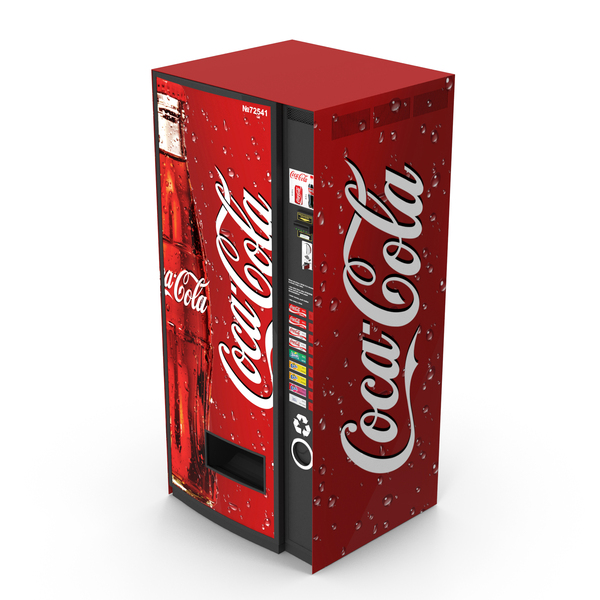
\includegraphics[width=16cm]{grafiki/automat.jpg}
    \caption{\footnotesize Automat \cite{www-1}}
\end{figure}

\addcontentsline{toc}{chapter}{Wstęp}
\newpage
% ********** Rozdział 1 **********
\chapter{Opis założeń i cele projektu}
\section{Cel projektu}



Celem projektu jest stworzenie kompleksowego systemu informatycznego symulującego działanie automatu z napojami. Głównym celem jest usprawnienie zarządzania produktami, transakcjami oraz operacjami administracyjnymi w systemie. Projekt zakłada zautomatyzowanie kluczowych procesów, takich jak zakup produktów, obsługa płatności, zarządzanie stanem automatu oraz funkcje administracyjne, w tym zarządzanie asortymentem i przeglądanie transakcji. Realizacja projektu ma na celu poprawę efektywności operacji, zapewnienie intuicyjnej obsługi użytkownika oraz stworzenie stabilnego środowiska do zarządzania automatem vendingowym.



\section{Opis założeń}

Poniższe założenia mają na celu stworzenie funkcjonalnego systemu symulującego automat vendingowy, który umożliwi łatwe zarządzanie produktami, transakcjami oraz operacjami administracyjnymi, zapewniając jednocześnie przyjazną obsługę dla użytkownika.

\begin{itemize}
\item \textbf{Zarządzanie asortymentem}: System umożliwia pełne zarządzanie produktami dostępnymi w automacie z napojami. Administrator może dodawać nowe produkty, aktualizować ceny, modyfikować dostępne ilości oraz usuwać produkty, które nie są już potrzebne.

\item \textbf{Obsługa transakcji}: System zapewnia płynne przetwarzanie zakupów dokonywanych przez użytkowników. Pozwala na realizację transakcji w czasie rzeczywistym, obsługę płatności, wydawanie reszty oraz zapisywanie historii zakupów w bazie danych.

\item \textbf{Obsługa klienta}: Projekt zakłada intuicyjny interfejs użytkownika, który pozwala na łatwy wybór produktów, dokonywanie płatności oraz korzystanie z prostych komunikatów systemowych. 

\item \textbf{Panel administracyjny}: System oferuje dedykowany panel dla administratorów, który umożliwia przeglądanie transakcji, monitorowanie stanu automatu, zarządzanie środkami pieniężnymi w urządzeniu oraz dokonywanie wypłat gotówki z automatu.

\item \textbf{Bezpieczeńwość danych}: System uwzględnia odpowiednie mechanizmy zabezpieczeń, takie jak hasła dla panelu administratora oraz walidacja danych wejściowych, aby zapewnić ochronę przed błędami lub nadużyciami.

\item \textbf{Efektywność operacyjna}: Celem projektu jest stworzenie niezawodnego i łatwego w utrzymaniu systemu, który zautomatyzuje kluczowe procesy, zmniejszy ryzyko błędów i usprawni zarządzanie automatem vendingowym.

\item \textbf{Skalowalność}: Projekt został stworzony z myślą o łatwej rozbudowie i adaptacji, aby sprostać rosnącym wymaganiom i zmieniającym się potrzebom.

\end{itemize}








\newpage
% ********** Rozdział 2 **********
\chapter{Funkcjonalności i niefunkcjonalności}

\section{Wymagania funkcjonalne:}
\begin{itemize}
       
    \item \textbf{Obsługa zamówień:}
    \begin{itemize}
        \item Umożliwia wybór produktów przez użytkownika.
        \item Obsługuje proces zakupu z automatycznym rozliczaniem płatności.
        \item Informuje o dostępności produktów w automacie.
        \item Wyświetla szczegóły transakcji, takie jak reszta i potwierdzenie zakupu.
    \end{itemize}
    
    \item \textbf{Obsługa klienta:}
    \begin{itemize}
        \item Zapewnia prosty interfejs dla użytkowników do zakupu produktów.
        \item Umożliwia poprawną obsługę wyjątków, takich jak brak produktu czy błędne dane.
        \item Umożliwia użytkownikom interakcję z systemem w intuicyjny sposób.
    \end{itemize}
    
    \item \textbf{Logistyka i dostawy:}
    \begin{itemize}
        \item Śledzi dostępność produktów w automacie.
        \item Zarządza stanem magazynowym automatów.
        \item Umożliwia szybkie uzupełnianie brakujących produktów.
    \end{itemize}
    
    \item \textbf{Bezpieczeństwo danych:}
    \begin{itemize}
        \item Chroni dane użytkowników i transakcji przed utratą i błędami.
        \item Stosuje mechanizmy weryfikacji dostępu do panelu administracyjnego.
    \end{itemize}
    
    \item \textbf{Zarządzanie asortymentem:}
    \begin{itemize}  
        \item Pozwala administratorowi na dodawanie, edytowanie i usuwanie produktów.
        \item Aktualizuje ceny i stany magazynowe w czasie rzeczywistym.
    \end{itemize}
\end{itemize}

\newpage

\section{Wymagania niefunkcjonalne:}
\begin{itemize}
    \item \textbf{Wydajność:}
    \begin{itemize}
        \item System działa płynnie i szybko, nawet podczas intensywnego użytkowania.    
    \end{itemize}

    
    \item \textbf{Dostępność:}
    \begin{itemize}
        \item System powinien być dostępny 24/7 z minimalnymi przerwami na konserwację.
    \end{itemize}


    
    \item \textbf{Skalowalność:}
    \begin{itemize}
        \item System powinien być łatwo skalowalny, aby dostosować się do wzrostu liczby klientów i transakcji.
    \end{itemize}
    
    \item \textbf{Bezpieczeństwo:}
    \begin{itemize}
        \item Zapewnienie ochrony danych transakcyjnych i dostępu administracyjnego.
    \end{itemize}
    
    \item \textbf{Interfejs użytkownika:}
    \begin{itemize}
        \item Przyjazny i intuicyjny interfejs użytkownika, który umożliwia łatwe nawigowanie i korzystanie z systemu.
    \end{itemize}
    
    \item \textbf{Zgodność z przepisami:}
    \begin{itemize}
        \item System powinien spełniać wszystkie wymogi prawne i regulacje dotyczące przechowywania i przetwarzania danych osobowych oraz transakcji.
    \end{itemize}
    
    \item \textbf{Wsparcie technologiczne:}
    \begin{itemize}
        \item System powinien być oparty na nowoczesnych technologiach i frameworkach, aby zapewnić stabilność, bezpieczeństwo i skalowalność.
    \end{itemize}
\end{itemize}






% ********** Koniec rozdziału **********

\newpage

 % ********** Rozdział 3 **********

\chapter{Opis projektu}
\section{Opis struktury projektu}

\subsection{Diagram klas}


\begin{figure}[H] % Użyto opcji H
    \centering
    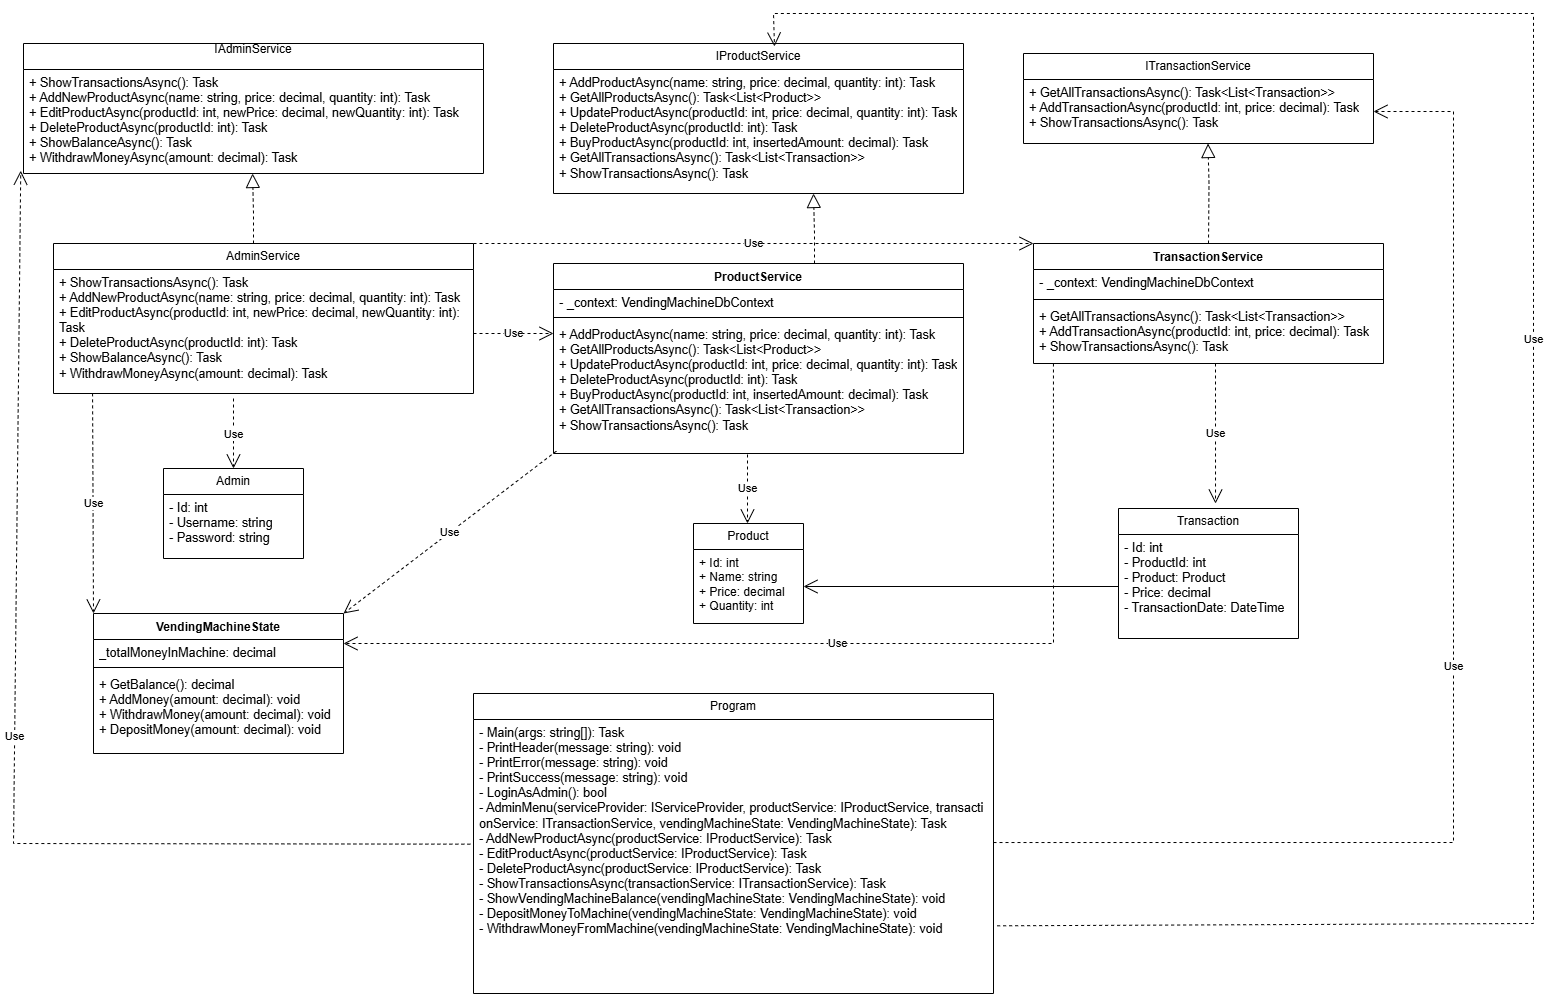
\includegraphics[width=1\textwidth ]{grafiki/diag_klas.PNG}
    \caption{\footnotesize Diagram przedstawiający strukturę klas programu}	
\end{figure}
\newpage

\subsection{Struktura diagramu klas}

Struktura diagramu klas przedstawia zależności między klasami, ich funkcje oraz relacje. Każda klasa ma określoną rolę w symulacji działania automatu z napojami i współpracuje z innymi klasami, aby zapewnić kompleksowe doświadczenie użytkownika, zarządzanie zapasami, obsługę transakcji oraz administrowanie stanem automatu.

\subsubsection*{Program}
Klasa główna aplikacji, która zarządza działaniem całego systemu. Odpowiada za uruchomienie aplikacji, obsługę interakcji użytkownika, takich jak wybór opcji z menu, zakupy, zarządzanie stanem automatu i wyświetlanie komunikatów. Korzysta z różnych serwisów, takich jak AdminService, TransactionService i ProductService, aby zapewnić poprawne działanie aplikacji.

\subsubsection*{AdminService}
Klasa zarządzająca administracyjnymi funkcjami aplikacji. Odpowiada za zarządzanie zapasami produktów w automacie, aktualizowanie stanów produktów, sprawdzanie dostępności towarów oraz monitorowanie transakcji. AdminService komunikuje się z klasami ProductService i TransactionService w celu zarządzania zapasami i obsługi transakcji. Ponadto korzysta z klasy VendingMachineState do monitorowania stanu maszyny.

\subsubsection*{TransactionService}
Klasa odpowiedzialna za obsługę transakcji w aplikacji. Zajmuje się realizowaniem zakupów, obliczaniem wydawanej reszty oraz zapisami transakcji. TransactionService współpracuje z klasą ProductService w celu obliczania kosztów produktów i aktualizowania zapasów, oraz z klasą Transaction w celu rejestrowania szczegółów transakcji.

\subsubsection*{ProductService}
Klasa odpowiedzialna za zarządzanie produktami w automacie vendingowym. Umożliwia dodawanie nowych produktów, usuwanie ich, edytowanie cen i dostępnych ilości. ProductService współpracuje z AdminService, aby zapewnić aktualizację zapasów w automacie i umożliwia przechowywanie informacji o produktach w bazie danych.

\subsubsection*{VendingMachineState}
Zarządza stanem maszyny, takim jak dostępne monety, zapasy produktów i ogólny stan operacyjny. Wykorzystywana przez AdminService i TransactionService.

\subsubsection*{Transaction}
Klasa reprezentująca pojedynczą transakcję w systemie. Zawiera informacje o dokonanym zakupie, takich jak zakupiony produkt, jego cena, kwota zapłacona przez klienta, reszta oraz status transakcji. Transaction jest używana przez TransactionService do przechowywania szczegółów transakcji oraz współpracuje z Product w celu aktualizacji zapasów po dokonaniu zakupu.

\subsubsection*{Product}
Klasa reprezentująca pojedynczy produkt w automacie vendingowym. Zawiera dane dotyczące produktu, takie jak jego nazwa, cena, ilość w zapasie i unikalny identyfikator. Product jest używana przez ProductService do zarządzania informacjami o produktach oraz przez TransactionService do obliczania kosztów produktów w transakcjach.



\section{Opis techniczny projektu}


\subsection{Język programowania:}
Projekt został zaimplementowany w języku C\# .NET 7.0 (Console App).

\subsection{Narzędzia:}
\begin{itemize}
    \item Środowisko programistyczne: Projekt był rozwijany w środowisku Visual Studio, które zapewnia wsparcie dla tworzenia aplikacji w języku C\# oraz ułatwia zarządzanie projektem.
    \item Baza danych: Aplikacja korzysta z SQL Server jako systemu zarządzania bazą danych, a do komunikacji z bazą użyto Entity Framework Core, zapewniając prostą integrację danych
\end{itemize}

\subsection{Minimalne wymagania sprzętowe:}
Minimalne wymagania sprzętowe dla uruchomienia aplikacji zależą głównie od zasobów potrzebnych do uruchomienia systemu operacyjnego oraz środowiska uruchomieniowego (.NET 7.0). Zazwyczaj są to:
\begin{itemize}
    \item Procesor: 1 GHz lub szybszy procesor (x86- lub x64-bitowy)
    \item Pamięć RAM: 1 GB dla systemów 32-bitowych lub 2 GB dla systemów 64-bitowych
    \item Dysk twardy: Minimum 5-10 MB wolnego miejsca na dysku twardym
    \item System operacyjny: Windows 7 lub nowszy
\end{itemize}


\subsection{Baza danych}
Baza danych \textit{VendingMachineDB} została zaprojektowana w celu przechowywania danych związanych z funkcjonowaniem systemu automatu z napojami. Zawiera tabele, które odpowiadają za przechowywanie informacji o produktach i transakcjach. Struktura bazy danych zapewnia efektywne zarządzanie i integrację danych.

Każda tabela posiada klucz główny, który gwarantuje unikalność rekordów, oraz klucze obce, które definiują relacje między tabelami. Taki układ bazy danych umożliwia łatwą manipulację danymi w kontekście działania automatu z napojami.

\subsubsection*{Tabela Product}
Zawiera dane dotyczące produktów dostępnych w automacie, w tym nazwę, cenę, ilość w zapasie oraz identyfikatory kategorii. Klucz ProductID zapewnia jednoznaczność rekordów i umożliwia powiązanie z transakcjami.

\subsubsection*{Tabela Transaction}
Zapisuje szczegóły transakcji, w tym identyfikator produktu, date i godzine dokonania zakupu, zapłaconą kwotę oraz resztę wydaną klientowi. Każda transakcja posiada unikalny identyfikator TransactionID.
.


\newpage
\chapter{Harmonogram realizacji projektu}

`\section{Diagram Ganta}
Diagram Gantta to narzędzie używane w zarządzaniu projektami do graficznego przedstawienia harmonogramu działań projektowych w formie tabeli. Składa się z osi czasu oraz listy zadań do wykonania. Każde zadanie jest reprezentowane przez pasek na osi czasu, który pokazuje jego planowaną długość trwania oraz jego pozycję względem innych zadań. 
\begin{figure}[H] % Użyto opcji H
    \centering
    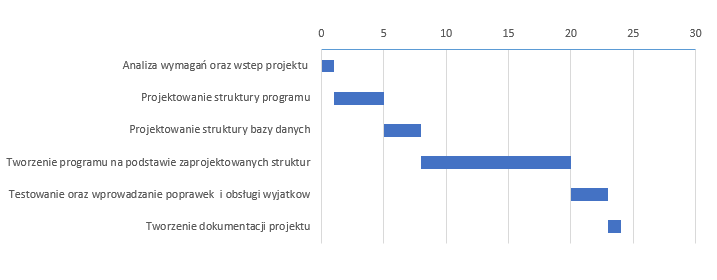
\includegraphics[width=0.8\textwidth]{grafiki/diag_ganta.PNG}
    \caption{\footnotesize Diagram przedstawiający harmonogram działań projektowych \cite{www-2}}
	\label{fig:plotend}
\end{figure}
\newpage
\section{Repozytorium i system kontroli wersji}

\begin{itemize}
    \item Repozytoria: GitHub umożliwia tworzenie repozytoriów, czyli przechowalni, w których można przechowywać pliki projektowe. Repozytoria mogą być publiczne, co oznacza, że są dostępne dla wszystkich, lub prywatne, dostępne tylko dla wybranych użytkowników.
    \item Zarządzanie zmianami: Dzięki systemowi kontroli wersji, takiemu jak Git, programiści mogą śledzić zmiany w kodzie, tworzyć gałęzie do eksperymentowania z nowymi funkcjami lub naprawami błędów, a następnie łączyć te zmiany z główną gałęzią, gdy są gotowe.
    \item Komentarze i dyskusje: Użytkownicy mogą komentować zmiany, zgłaszać problemy i prowadzić dyskusje na temat kodu lub innych plików w repozytorium.
    \item Kontrola dostępu: Właściciele repozytorium mogą kontrolować, kto ma dostęp do repozytorium i jakie uprawnienia mają użytkownicy, na przykład czy mogą zmieniać kod, zgłaszać problemy itp.
\end{itemize}
\subsection*{Github}
Projekt jest umieszczony w repozytorium: 
\newline
\href{https://github.com/DanielKaznowski/w69794_Automat_z_napojami}{\texttt{https://github.com/DanielKaznowski/w69794_Automat_z_napojami}}




% ********** Koniec rozdziału **********

\newpage
% ********** Rozdział 4 **********
\chapter{Warstwa użytkowa projektu}
\section{Menu główne}


Jest to główne menu aplikacji, które użytkownik widzi po uruchomieniu programu. Zapewnia dostęp do podstawowych funkcji systemu, takich jak dokonywanie zakupów, logowanie się na konto admina oraz wyjście z aplikacji. Użytkownik może poruszać się po opcjach menu za pomocą odpowiednich znaków.



\begin{figure}[H] 
    \centering
    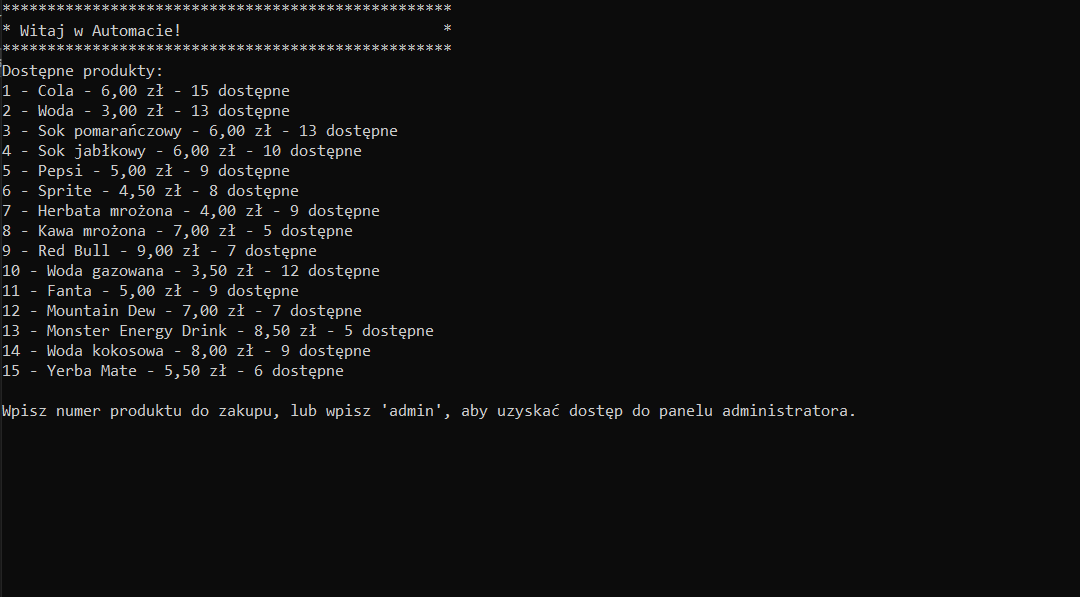
\includegraphics[width=0.8\textwidth]{grafiki/menu_glowne.PNG}
    \caption{\footnotesize Menu główne}	
\end{figure}

\newpage

\begin{figure}[H] 
    \centering
    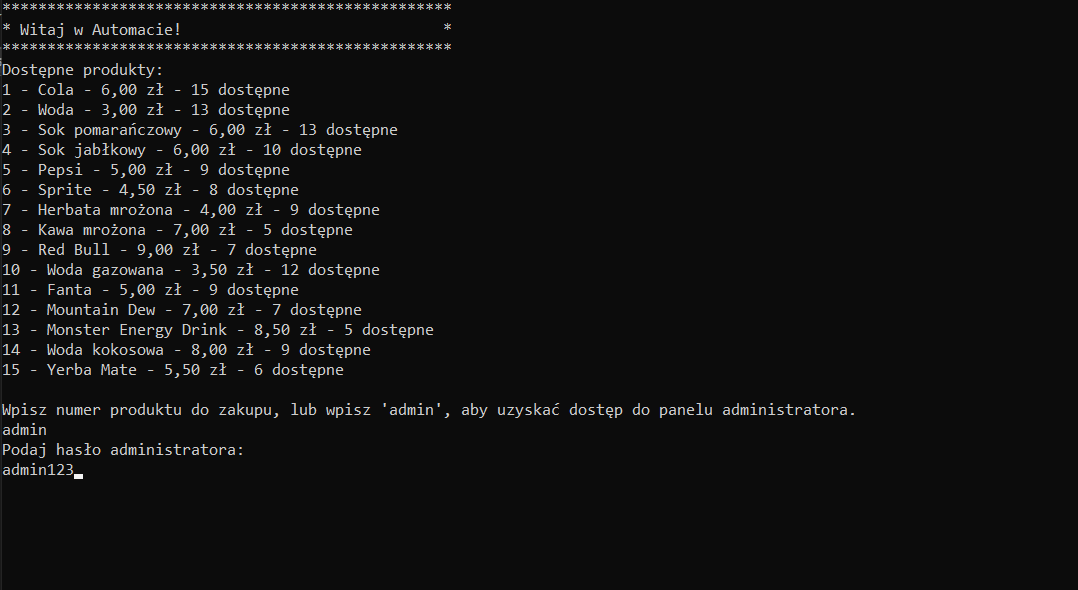
\includegraphics[width=0.8\textwidth]{grafiki/admin_log.png}
    \caption{\footnotesize Admin - logowanie}	
    \label{fig:5.2}

\end{figure}

Na rys. \ref{fig:5.2} Logowanie do panelu admina za pomocą hasła 

\begin{figure}[H] 
    \centering
    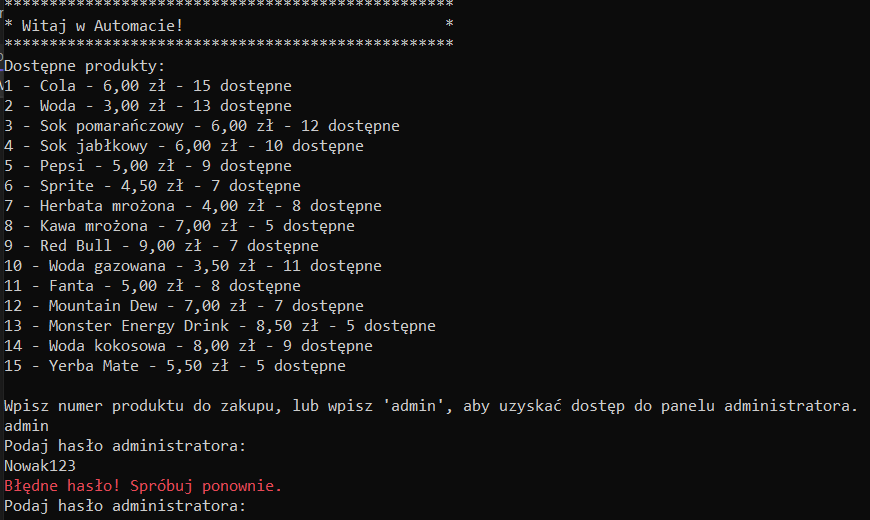
\includegraphics[width=0.8\textwidth]{grafiki/blad_admin_haslo1.png}
    \caption{\footnotesize Admin - logowanie błąd}	
    \label{fig:5.3}

\end{figure}

Na rys. \ref{fig:5.3} Widać błąd ponieważ hasło które zostało podane jest niepoprawne.

\newpage

\begin{figure}[H] 
    \centering
    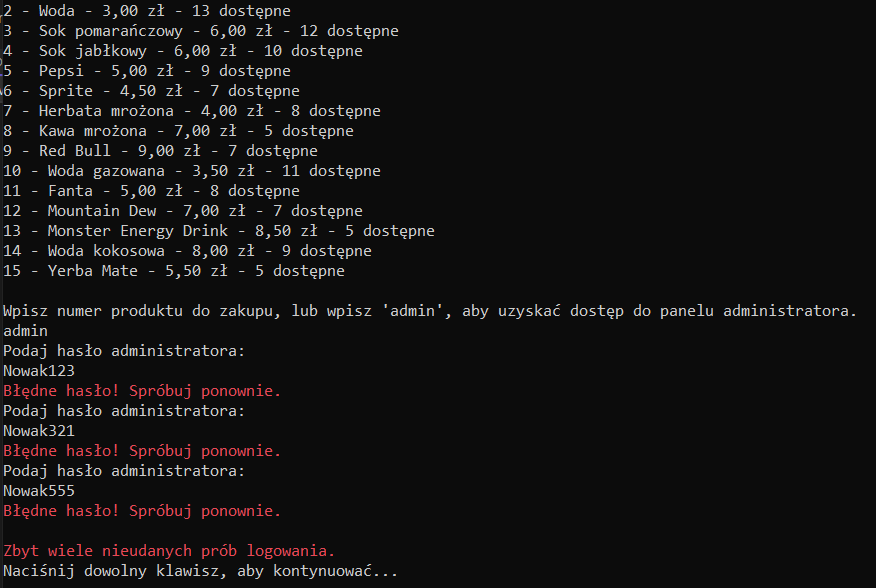
\includegraphics[width=0.8\textwidth]{grafiki/blad_admin_haslo2.png}
    \caption{\footnotesize Admin - logowanie 3 nieudane próby}	
    \label{fig:5.4}

\end{figure}

Na rys. \ref{fig:5.4} Gdy wprowadzone hasło będzie nieprawidłowe trzykrotnie wyświetli się komunikat o zbyt wielu nieudanych próbach logowania.

% ********************

\section{Zakup produktu}

 \begin{figure}[H] 
    \centering
    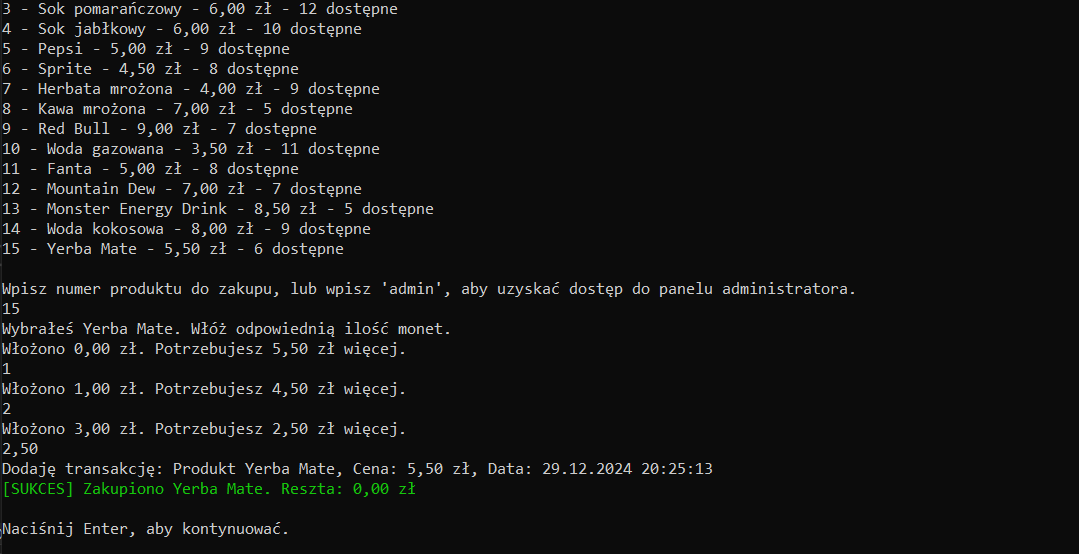
\includegraphics[width=0.8\textwidth]{grafiki/zakup_produktu_bez_reszty.png}
    \caption{\footnotesize Zakup produktu:}	
    \label{fig:5.5}
\end{figure}



Pozwala klientowi na prosty zakup produktu z listy a jeśli trzeba wydaje jego resztę.


\begin{figure}[H] 
    \centering
    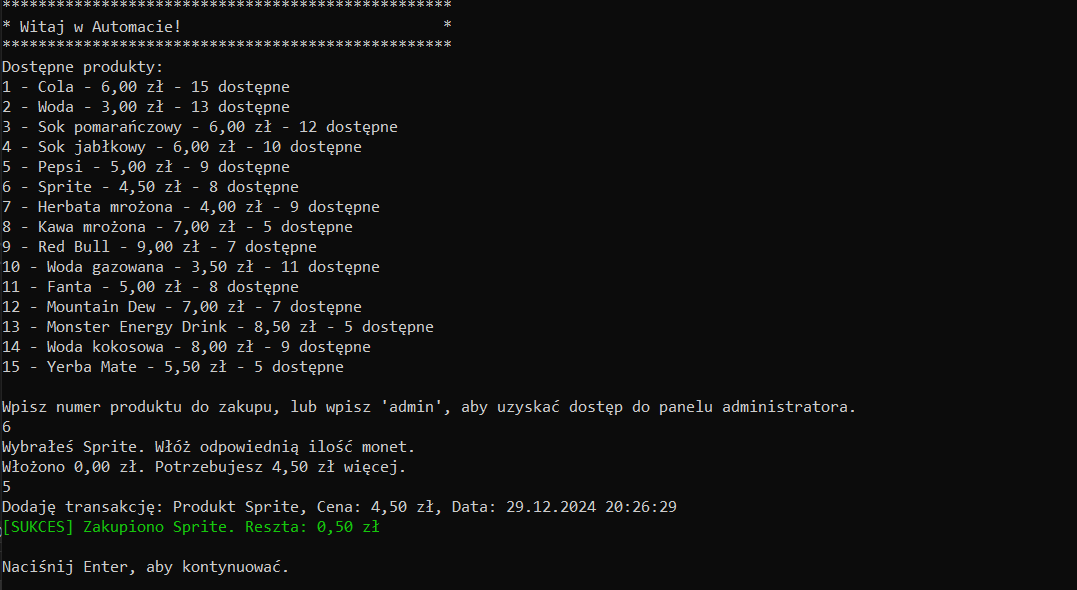
\includegraphics[width=0.8\textwidth]{grafiki/zakup_produktu_reszta.png}
    \caption{\footnotesize Zakup produktu - wydanie reszty dla klienta}	
    \label{fig:5.6}
\end{figure}

Jak widać podczas zakupu automat prosi klienta o podaną kwotę którą może wpłacać na raty a w razie potrzeby wydaje mu jego resztę oraz wyświetla się komunikat o sukcesie dokonania zakupu.



\begin{figure}[H] 
    \centering
    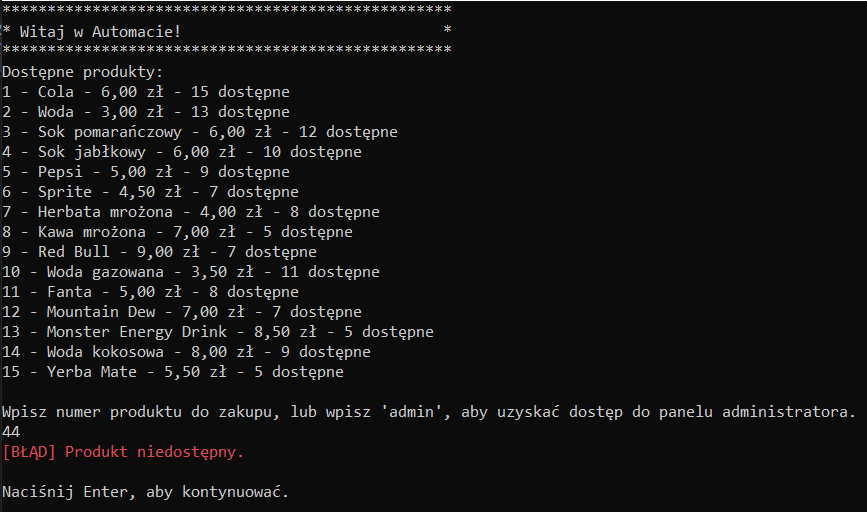
\includegraphics[width=0.8\textwidth]{grafiki/blad_zakupu.png}
    \caption{\footnotesize Zakup produktu - błędne ID}	
    \label{fig:5.7}
\end{figure}

Gdy wypiszemy błędne ID podczas zakupu dostaniemy informacje że produkt nie jest dostępny.


\newpage

 
\section{Menu admina}

Jest to menu, które umożliwia adminowi na dodawanie usuwanie oraz edytowanie produktów. Może on także wyświetlić listę transakcji, sprawdzić ile pieniędzy aktualnie znajduje się w automacie, wpłacić lub wypłacić pieniądze z automatu.

\begin{figure}[H] 
    \centering
    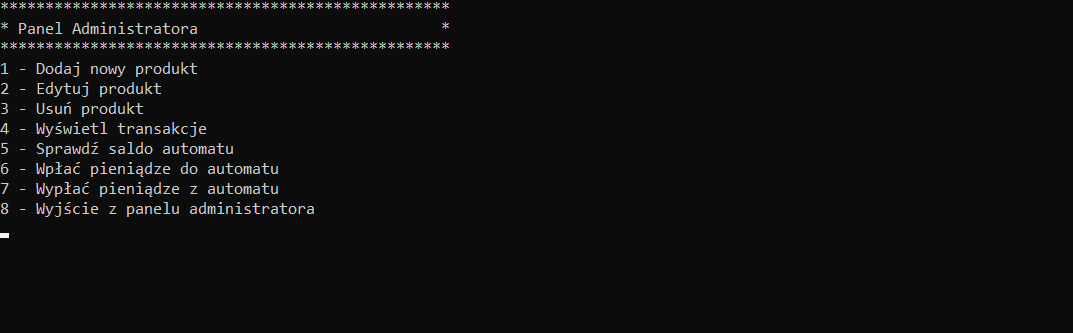
\includegraphics[width=0.8\textwidth]{grafiki/menu_admin.png}
    \caption{\footnotesize Menu admina}	
    \label{fig:5.8}
\end{figure}

W menu admina mamy do wyboru osiem opcji takich jak: dodanie nowego produktu, edycja produktu, usunięcie produktu, wyświetlenie transakcji, sprawdzenie salda, wpłacenie pieniędzy do automatu, wypłacenie pieniędzy z automatu oraz wyjście.



\begin{figure}[H] 
    \centering
    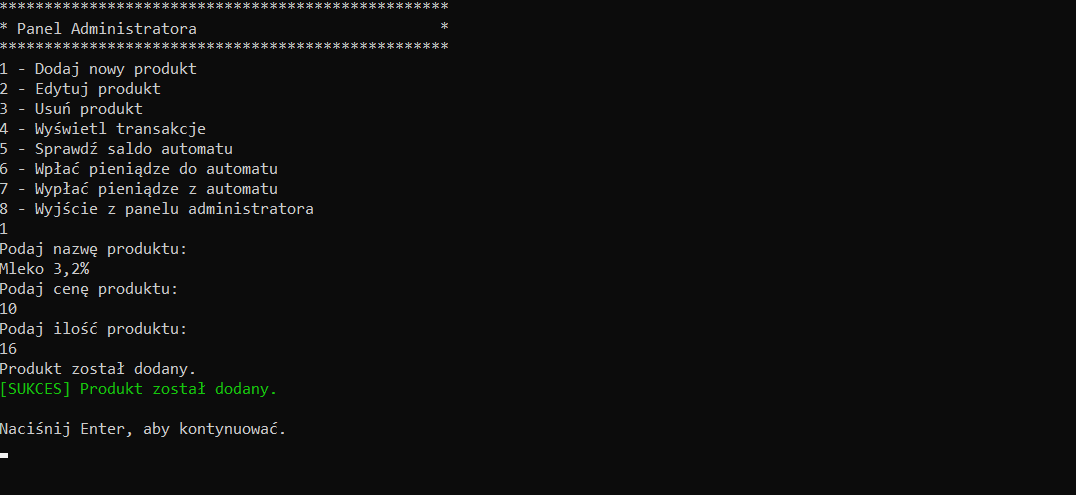
\includegraphics[width=0.8\textwidth]{grafiki/dodanie_produktu.png}
    \caption{\footnotesize Menu admina - dodanie produktu}	
    \label{fig:5.9}
\end{figure}
Aby dodać nowy produkt do automatu, konieczne jest podanie jego nazwy, ceny oraz dostępnej ilości. Każdy z tych parametrów jest niezbędny, aby produkt mógł zostać prawidłowo zapisany w systemie i udostępniony klientom.


\newpage


\begin{figure}[H] 
    \centering
    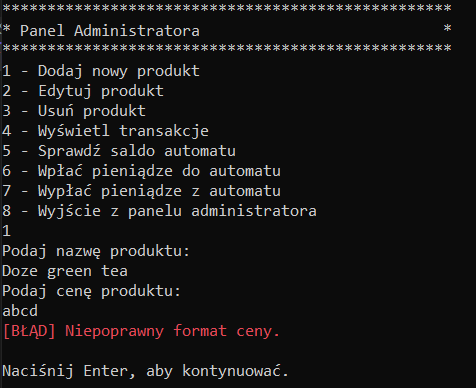
\includegraphics[width=0.8\textwidth]{grafiki/blad_format_ceny.png}
    \caption{\footnotesize Menu admina - dodanie produktu błąd formatu ceny}	
    \label{fig:5.10}
\end{figure}
Podczas wprowadzania ceny produktu należy upewnić się, że jej format jest prawidłowy. Cena powinna być zapisana jako wartość liczbowa z separatorami dziesiętnymi zgodnymi z przyjętym standardem. Nieprawidłowy format może uniemożliwić dodanie produktu lub prowadzić do błędów w działaniu systemu.

\newpage


\begin{figure}[H] 
    \centering
    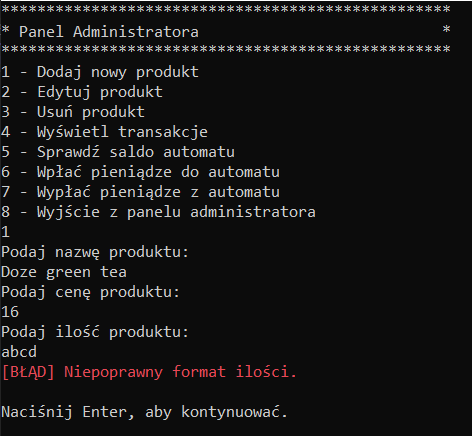
\includegraphics[width=0.8\textwidth]{grafiki/blad_format_ilosci.png}
    \caption{\footnotesize Menu admina - dodanie produktu błąd format ilości}	
    \label{fig:5.11}
\end{figure}
Przed zapisaniem nowego produktu w bazie danych należy sprawdzić, czy podana ilość jest poprawna. System akceptuje wyłącznie wartości liczbowe, które określają liczbę dostępnych sztuk danego produktu w automacie. Wprowadzenie błędnego formatu może skutkować nieprawidłowym działaniem aplikacji.

\newpage


\begin{figure}[H] 
    \centering
    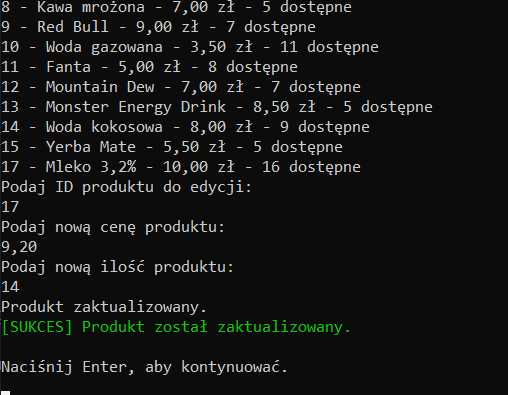
\includegraphics[width=0.8\textwidth]{grafiki/edycja_produktu.png}
    \caption{\footnotesize Menu admina - edycja produktu}	
    \label{fig:5.12}
\end{figure}
Jeśli chcemy edytować dane produktu, musimy najpierw wybrać jego unikalny identyfikator (ID). Następnie podajemy nową cenę oraz ilość, która ma zostać zaktualizowana w systemie. Warto pamiętać, aby upewnić się, że wprowadzane wartości są poprawne, ponieważ błędne dane mogą wpłynąć na dostępność i wycenę produktu w automacie.

\newpage

\begin{figure}[H] 
    \centering
    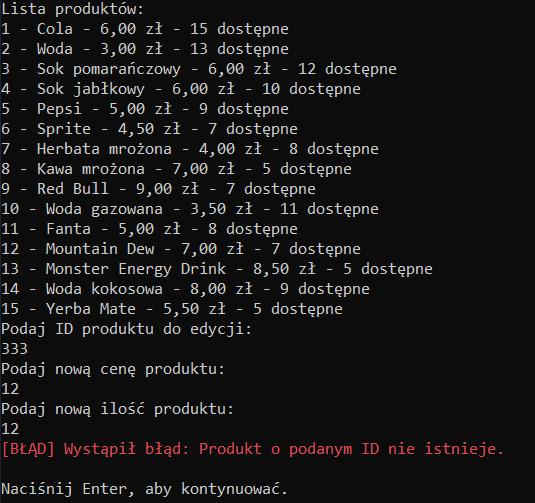
\includegraphics[width=0.8\textwidth]{grafiki/blad_id_edycja.png}
    \caption{\footnotesize Menu admina - edycja produktu błędne ID}	
    \label{fig:5.13}
\end{figure}
Na rys. \ref{fig:5.13} Podczas próby edycji produktu możemy zauważyć błąd wynikający z podania nieprawidłowego identyfikatora (ID). Oznacza to, że w systemie nie istnieje produkt o wskazanym ID, co uniemożliwia jego modyfikację.

\newpage

\begin{figure}[H] 
    \centering
    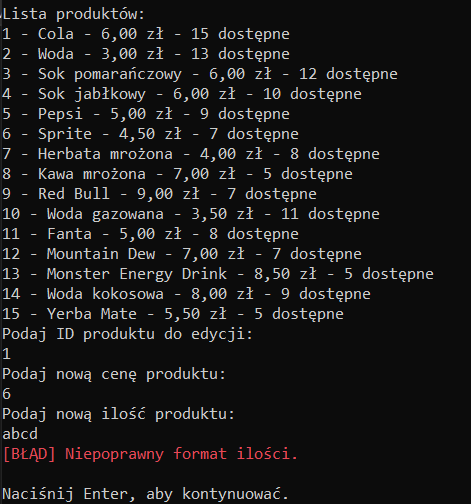
\includegraphics[width=0.8\textwidth]{grafiki/blad_ilosc_edycja.png}
    \caption{\footnotesize Menu admina - edycja produktu zły format ilości}	
    \label{fig:5.14}
\end{figure}
Na rys. \ref{fig:5.14} System zgłasza błąd, ponieważ podany format ilości produktu podczas edycji jest nieprawidłowy. Wartość ta powinna być liczbą całkowitą, oznaczającą dostępny stan magazynowy produktu w automacie. Niepoprawny format może skutkować błędnym działaniem systemu.

\newpage


\begin{figure}[H] 
    \centering
    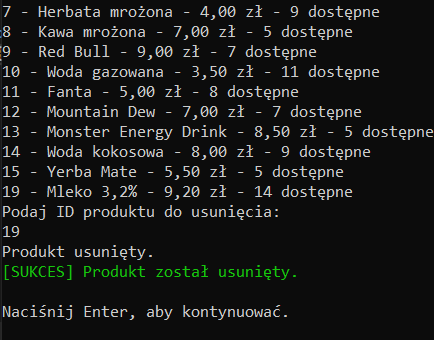
\includegraphics[width=0.8\textwidth]{grafiki/usun_produkt.png}
    \caption{\footnotesize Menu admina - usuwanie produktu}	
    \label{fig:5.15}
\end{figure}

Aby usunąć wybrany produkt z systemu, należy skorzystać z opcji "3 - Usuń produkt" w menu administratora. Następnie wymagane jest podanie poprawnego identyfikatora (ID) produktu znajdującego się na liście. Po potwierdzeniu operacji produkt zostanie usunięty z bazy danych.

\newpage

\begin{figure}[H] 
    \centering
    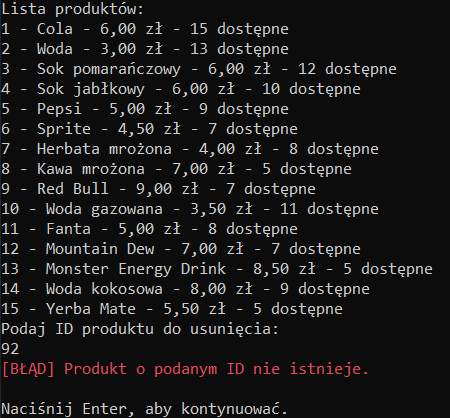
\includegraphics[width=0.8\textwidth]{grafiki/blad_id_usun.png}
    \caption{\footnotesize Menu admina - usuwanie produktu błąd}	
    \label{fig:5.16}
\end{figure}

Na rys. \ref{fig:5.16} W przypadku podania nieprawidłowego identyfikatora (ID) system nie pozwoli na usunięcie produktu. Jeśli dany ID nie istnieje w bazie, operacja zostanie przerwana, a użytkownik otrzyma stosowny komunikat o błędzie.

\newpage

\begin{figure}[H] 
    \centering
    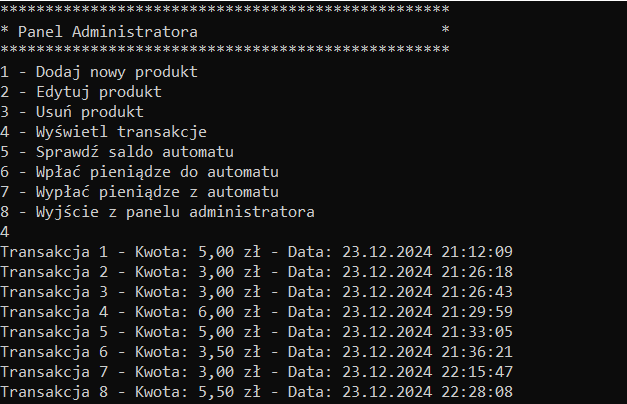
\includegraphics[width=0.8\textwidth]{grafiki/wyswietl_transakcje.png}
    \caption{\footnotesize Menu admina - wyświetl transakcje}	
    \label{fig:5.17}
\end{figure}

Po wybraniu opcji "4 - Wyświetl transakcje" uzyskujemy dostęp do historii dokonanych transakcji w automacie z napojami. Dzięki temu administrator może przeanalizować wcześniejsze zakupy użytkowników.

\begin{figure}[H] 
    \centering
    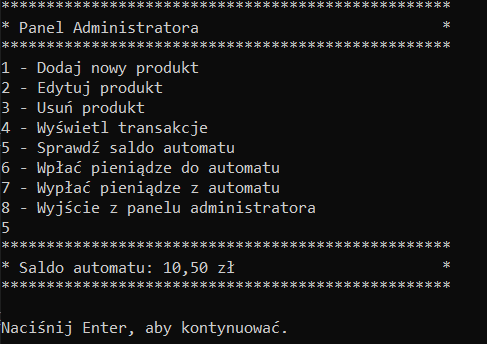
\includegraphics[width=0.8\textwidth]{grafiki/saldo_automatu.png}
    \caption{\footnotesize Menu admina - saldo automatu}	
    \label{fig:5.18}
\end{figure}

Aplikacja pozwala też na sprawdzenie salda automatu.

\newpage

\begin{figure}[H] 
    \centering
    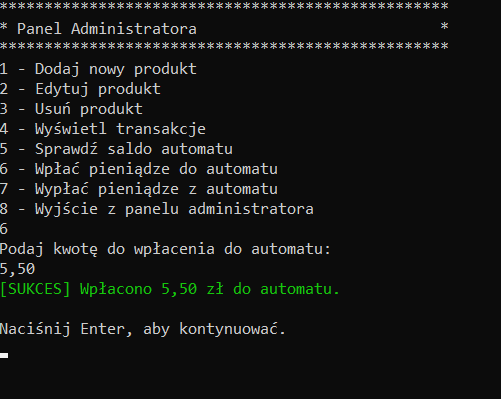
\includegraphics[width=0.8\textwidth]{grafiki/wplacanie_automat.png}
    \caption{\footnotesize Menu admina - dodawanie salda automatu}	
    \label{fig:5.19}
\end{figure}

Gdy automat jest pusty możemy wpłacić pieniądze żeby maszyna mogła wydawać resztę.

\begin{figure}[H] 
    \centering
    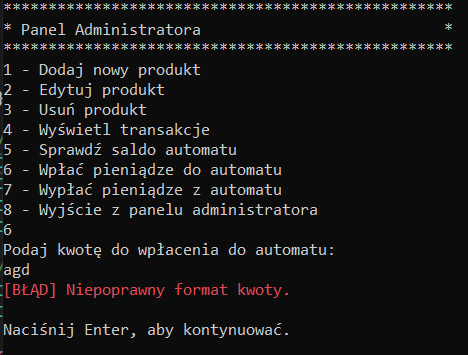
\includegraphics[width=0.8\textwidth]{grafiki/blad_wplata.png}
    \caption{\footnotesize Menu admina - dodawanie salda automatu}	
    \label{fig:5.20}
\end{figure}

Na rys. \ref{fig:5.20} Podczas wpłacania pieniędzy do automatu należy upewnić się, że wprowadzony format kwoty jest poprawny. W przeciwnym razie system wyświetli błąd.

\begin{figure}[H] 
    \centering
    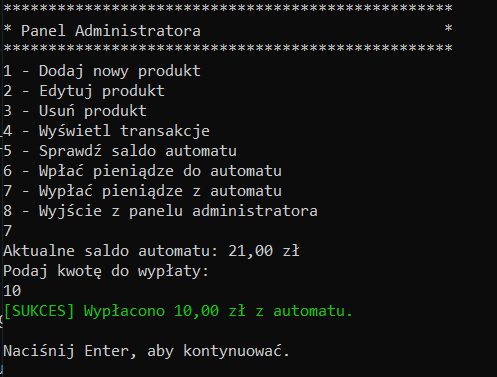
\includegraphics[width=0.8\textwidth]{grafiki/wyplacanie_pieniedzy.png}
    \caption{\footnotesize Menu admina - wyciąganie pieniędzy z automatu}	
    \label{fig:5.21}
\end{figure}

Aplikacja posiada też funkcję wypłaty pieniędzy z automatu.

\begin{figure}[H] 
    \centering
    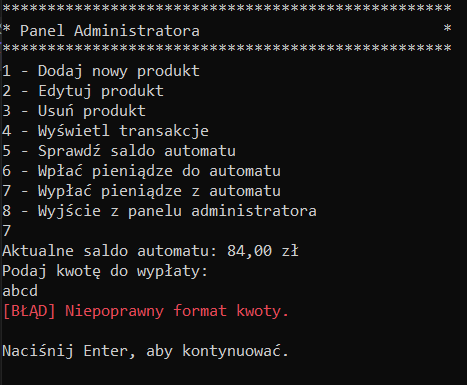
\includegraphics[width=0.8\textwidth]{grafiki/blad_format_wyplac.png}
    \caption{\footnotesize Menu admina - wyciąganie pieniędzy z automatu błąd formatu}	
    \label{fig:5.22}
\end{figure}

Aplikacja sprawdza czy format kwoty podczas wypłaty jest poprawny.

\begin{figure}[H] 
    \centering
    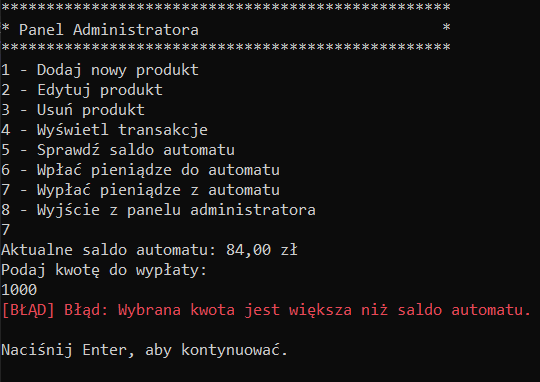
\includegraphics[width=0.8\textwidth]{grafiki/blad_kwota_wyplac.png}
    \caption{\footnotesize Menu admina - wyciąganie pieniędzy z automatu błąd formatu}	
    \label{fig:5.23}
\end{figure}

Jeśli kwota którą chcemy wyciągnąć jest większa niż saldo automatu to wystąpi błąd.



\chapter{Podsumowanie}

\section{Podsumowanie}
Aplikacja automatu z napojami oferuje kompleksowe rozwiązania umożliwiające zarządzanie produktami, transakcjami, stanem automatu oraz obsługą błędów. Główne menu zapewnia łatwy wybór i zakup produktu. Panel administratora pozwala na rzeczy takie jak dodawanie, edytowanie oraz usuwanie produktu. Pozwala nam także na przeglądanie historii transakcji, zarządzanie saldem automatu oraz wyjście z aplikacji. Logowanie zapewnia bezpieczny dostęp do systemu, a admin może efektywnie zarządzać automatem. Dzięki tym funkcjom aplikacja pozwala na poprawę obsługi klienta oraz optymalizację operacji związanych z zarządzaniem maszyną.

\section{Dalszy rozwój projektu}

Projekt automatu z napojami może być rozbudowywany w różnych kierunkach, aby zwiększyć jego funkcjonalność i użyteczność. Jednym z możliwych kierunków jest zwiększenie poziomu bezpieczeństwa aplikacji, np. poprzez dodanie bardziej zaawansowanych mechanizmów autentykacji lub szyfrowania danych użytkowników.

Dodatkowo, warto rozważyć implementację funkcji importowania i eksportowania danych z plików XLS lub CSV, co umożliwiłoby łatwe zarządzanie danymi, takimi jak zapasy produktów, transakcje czy raporty o stanie maszyny. Taka funkcjonalność pozwoliłaby na lepszą integrację aplikacji z systemami zewnętrznymi i ułatwiłaby obsługę dużych zbiorów danych.

Kolejnym obszarem rozwoju może być dodanie mechanizmu promocji, który umożliwiłby użytkownikom korzystanie z różnych ofert rabatowych lub zniżek na produkty. Może to zwiększyć zaangażowanie klientów i poprawić wyniki sprzedaży.

Warto również rozważyć integrację z nowoczesnymi metodami płatności, takimi jak portfele cyfrowe, płatności mobilne czy karty lojalnościowe, co poprawiłoby wygodę korzystania z automatu i zapewniłoby większą elastyczność w dokonywaniu płatności.
% ********** Koniec rozdziału **********
\newpage

% *************** Bibliografia ***************
\begin{thebibliography}{6}
\addcontentsline{toc}{chapter}{Bibliografia}
%dodanie wpisu do spisu bibliograficznego


\bibitem{www-2} https://www.youtube.com/watch?v=5T2DXFbSd18 
\bibitem{} Jacek Matulewski, C\#: lekcje programowania: praktyczna nauka programowania dla platform .NET i .NET Core, Helion, Gliwice 2021 
\bibitem{} Joseph  Albahari, Eric Johannsen, C\# 8.0 w pigułce, Helion, Gliwice, 2021
\bibitem{} R. S. Miles, C\#: zacznij programować!, Helion, Gliwice, 2020
\bibitem{} Włodzimierz Gajda, Git : rozproszony system kontroli wersji, Gliwice : Wydawnictwo Helion, 2013

\end{thebibliography}
\newpage

% *************** Zakończenie ***************
%spis rysunków
\addcontentsline{toc}{chapter}{Spis rysunków}
\listoffigures
\newpage


%streszczenie
\addcontentsline{toc}{chapter}{Streszczenie}
\noindent
{\footnotesize{}\textbf{Wyższa Szkoła Informatyki i Zarządzania z siedzibą w Rzeszowie\\
Kolegium Informatyki Stosowanej}
\vspace{30pt}

\begin{center}
\textbf{Streszczenie pracy dyplomowej inżynierskiej}\\
\temat
\end{center}

\vspace{30pt}
\noindent
\textbf{Autor: \autor
\\Promotor: \promotor
\\Słowa kluczowe: Automat z napojami, C\#, SQL Server }
\vspace{40pt}
\\Celem projektu jest stworzenie kompleksowego systemu informatycznego wspomagającego zarządzanie automatami z napojami, który umożliwia użytkownikom przeglądanie, wybieranie i zakup produktów dostępnych w maszynach. Projekt zakłada usprawnienie zarządzania stanem maszyn, ich asortymentem oraz procesami związanymi z obsługą klienta. Założenia projektu obejmują m.in. zarządzanie produktami, obsługę transakcji, bezpieczeństwo danych, generowanie raportów oraz import/eksport danych. Projekt ma na celu zautomatyzowanie wielu procesów, poprawę obsługi klienta oraz optymalizację kosztów operacyjnych. \newline
Projekt został zaimplementowany w języku C\# (.NET 7.0) przy użyciu narzędzi takich jak Visual Studio do programowania oraz SQL Server do przechowywania danych aplikacji. Minimalne wymagania sprzętowe dla uruchomienia aplikacji obejmują m.in. procesor 1 GHz, pamięć RAM 1-2 GB oraz system operacyjny Windows 7 lub nowszy. \newline
Struktura bazy danych składa się z kilku tabel, zapewniając efektywne przechowywanie i zarządzanie danymi związanych z funkcjonowaniem automatów vendingowych.
\vspace{80pt}

\noindent
\textbf{The University of Information Technology and Management in Rzeszow\\
Faculty of Applied Information Technology}
\vspace{30pt}

\begin{center}
\textbf{Thesis Summary\\}
Drink Vending Machine Application
\end{center}

\vspace{30pt}
\noindent
\textbf{Author: \autor
\\Supervisor: \promotor
\\Key words: Drink Vending Machine, C\#, SQL Server}
\vspace{40pt}
\\The aim of the project is to create a comprehensive IT system supporting the management of vending machines, which allows users to browse, select, and purchase products available in the machines. The project aims to improve the management of machine statuses, their inventory, and processes related to customer service. The project's assumptions include, among others, product management, transaction handling, data security, report generation, and data import/export. The project is designed to automate many processes, improve customer service, and optimize operational costs. \newline
The project was implemented in C\# (.NET 7.0) using tools such as Visual Studio for programming and SQL Server for storing application data. The minimum hardware requirements to run the application include a 1 GHz processor, 1-2 GB RAM, and a Windows 7 or newer operating system. \newline
The database structure consists of several tables, ensuring efficient storage and management of data related to the operation of the vending machines.
}


\end{document}
% *************** Koniec pliku szablon.tex ***************
